% Fixture: linked
% hyperref turns every \cite, \ref and \eqref into an internal link
% annotation and writes an outline. The body is shared with `unlinked`.
\documentclass[10pt]{article}
% Shared settings for every Tourmaline fixture. \input this right after
% \documentclass.
%
% Reproducible output: no creation date, no random trailer id, no pdfTeX
% banner, so rebuilding with the same TeX Live gives byte-identical PDFs.
\pdfinfoomitdate=1
\pdftrailerid{}
\pdfsuppressptexinfo=-1
% Map every glyph (including the fi/fl/ffi ligatures) to Unicode so that
% text extraction does not depend on font-specific guesswork.
\input{glyphtounicode}
\pdfgentounicode=1

\usepackage[a4paper,margin=25mm]{geometry}
\usepackage{amsmath}
\usepackage{float}
\usepackage{tikz}
\usepackage[colorlinks,linkcolor=blue,citecolor=blue,bookmarksnumbered]{hyperref}
% Shared body of the `linked` and `unlinked` fixtures. Both documents use the
% same class, geometry and fonts and differ only in whether hyperref is
% loaded, so their pagination and text are identical; only `linked` has link
% annotations. Every page ends with an explicit \clearpage.
\title{Citation Previews in a Research Reader}
\author{Fay Instance\\ School of Worked Examples}
\date{}

\begin{document}
\maketitle

\begin{abstract}
Following a citation or a figure reference in a PDF usually means leaving the
current page. We describe a reader that shows the target in a small preview
instead, and compare two ways of finding the target: following the link
annotations that the typesetting system wrote into the file, and searching the
text for patterns such as bracketed numbers when no links exist.
\end{abstract}

% ------------------------------------------------------------------- page 1
\section{Introduction}\label{sec:intro}

Reference previews are an old idea in hypertext systems~\cite{nelson} and
have been studied for web pages and wikis~\cite{wiki,hover}. For scholarly
PDFs the situation is less settled, because many files carry no link
annotations at all and the reader has to recover the structure from the
text alone.

The model we use is summarised in Section~\ref{sec:model}, and the preview
pipeline is shown in Figure~\ref{fig:pipeline} on the next page.

\section{Model}\label{sec:model}

We score a candidate target $t$ for a reference $r$ by combining a textual
match with a penalty for distance in the document:
\begin{equation}
  s(r,t) = m(r,t) - \lambda\, d(r,t) .
  \label{eq:score}
\end{equation}
The textual match is one when the label of the target equals the visible
text of the reference and zero otherwise. The distance is counted in pages,
and the weight is chosen so that an exact match always wins:
\begin{equation}
  0 < \lambda < \frac{1}{N} .
  \label{eq:lambda}
\end{equation}

\clearpage
% ------------------------------------------------------------------- page 2
\begin{figure}[H]
  \centering
  \begin{tikzpicture}[x=10mm,y=10mm]
    \draw (0,0) rectangle (3,1.2);
    \draw (4.5,0) rectangle (7.5,1.2);
    \draw (9,0) rectangle (12,1.2);
    \draw[->,thick] (3,0.6) -- (4.5,0.6);
    \draw[->,thick] (7.5,0.6) -- (9,0.6);
  \end{tikzpicture}
  \caption{The preview pipeline: detect the reference, locate its target,
  and render the target region in a popup.}
  \label{fig:pipeline}
\end{figure}

\section{Experiments}\label{sec:experiments}

We ran the scoring rule of Eq.~\eqref{eq:score} on a set of papers with and
without link annotations. Link annotations were present in most recent
papers, in line with earlier surveys~\cite{survey}, but almost absent from
scanned and older material~\cite{scan,ocr}. The resulting accuracy is shown
in Figure~\ref{fig:accuracy}.

\begin{figure}[H]
  \centering
  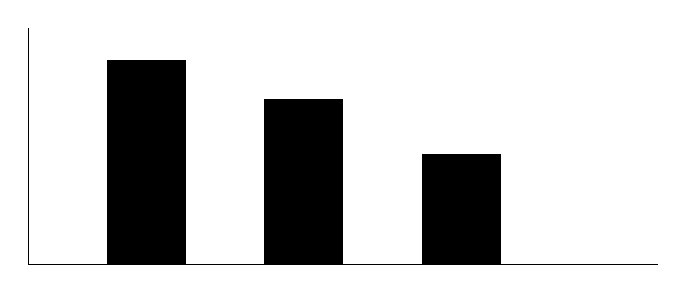
\begin{tikzpicture}[x=10mm,y=10mm]
    \draw (0,0) -- (8,0);
    \draw (0,0) -- (0,3);
    \fill (1,0) rectangle (2,2.6);
    \fill (3,0) rectangle (4,2.1);
    \fill (5,0) rectangle (6,1.4);
  \end{tikzpicture}
  \caption{Accuracy of target detection for linked papers, unlinked papers
  and scanned papers after text recognition.}
  \label{fig:accuracy}
\end{figure}

\section{Discussion}\label{sec:discussion}

The bound in Eq.~\eqref{eq:lambda} matters most for unlinked papers, where
the same label can occur more than once. As argued in
Section~\ref{sec:intro}, links should be preferred whenever they exist; the
text patterns of Fig.~\ref{fig:pipeline} are a fallback. Similar fallbacks
are used by reference managers~\cite{manager} and by accessibility
tools~\cite{access}.

\clearpage
% ------------------------------------------------------------------- page 3
\begin{thebibliography}{9}
\bibitem{nelson} T. Example. Links that show their targets. \emph{Journal of
  Hypothetical Hypertext}, 3(1):1--12, 1975.
\bibitem{wiki} U. Sample and V. Model. Hover previews in collaborative
  encyclopedias. In \emph{Proceedings of the Placeholder Conference},
  pages 10--18, 2016.
\bibitem{hover} W. Instance. Measuring the cost of a click. \emph{Notes on
  Imaginary Interfaces}, 7:44--51, 2018.
\bibitem{survey} X. Filler, Y. Dummy and Z. Mock. A survey of link
  annotations in scholarly files. Technical report, Fixture Institute, 2020.
\bibitem{scan} A. Scanner. Old papers as images. \emph{Archive Studies
  Quarterly}, 15(2):100--120, 2012.
\bibitem{ocr} B. Reader. Recognising text in degraded page images. In
  \emph{Workshop on Invented Methods}, pages 1--8, 2014.
\bibitem{manager} C. Keeper. Reference managers and the PDF. \emph{Library
  Tools Review}, 22:5--30, 2019.
\bibitem{access} D. Helper. Accessible navigation of long documents.
  \emph{Journal of Sample Accessibility}, 9(4):200--215, 2021.
\end{thebibliography}

\end{document}

